\section{Example: The Dining Philosophers}

The Dining Philosophers problem is an example formulated by Edsger Dijkstra
to illustrate some of the problems that can arise in concurrent programming.  
It is presented in terms of interactions between people; but it is an analogy
for concurrent threads or processes sharing resources. 

Five philosophers spend most of their lives thinking; but sometimes they need
to eat.  They share a common dining room, which has a circular table with five
chairs around it, a plate in front of each chair, and a big bowl of spaghetti
in the middle.  There are five forks, placed between the five plates at the
table; a philosopher needs two forks in order to eat the spaghetti. 

When a philosopher gets hungry, they sit down.  They pick up the fork to their
left as soon as it's available (they might need to wait for their left-hand
neighbour to finish with the fork).  Then they pick up the fork to their right
as soon as it's available.  Once the philosopher has two forks, they serve
themself and spend some time eating.  The philosopher then puts the forks
down, leaves the table, and does some more thinking.

However, there is a problem with this protocol.  If all five philosophers get
hungry at about the same time and pick up their left fork, then they are
unable to obtain their right fork, and so all starve!  Of course, real
philosophers---being smart people---would soon solve the problem.  But if we
think of this as an analogy for concurrent threads, the program would not.

We will build a simulation of the Dining Philosophers example.  We 
simulate each philosopher and each fork by a thread.  The first part of the
simulation is in Figure~\ref{fig:dining-phils-1}.  We denote the number of
philosophers by~|N|; this allows us to easily vary the number. 

%%%%%%%%%%

\begin{figure}
\begin{scala}
/** Simulation of the Dining Philosophers example. */
object Phils{
  val N = 5 // Number of philosophers.

  // Simulate basic actions.
  def eat() = Thread.sleep(500)
  def think() = Thread.sleep(scala.util.Random.nextInt(900))
  def pause() = Thread.sleep(500)

  type Cmd = Boolean; val Pick = true; val Drop = false
 
  /** A single philosopher. */
  def phil(me: Int, left: !![Cmd], right: !![Cmd]) = thread(s"Phil $me"){
    repeat{
      think()
      println(s"$me sits"); pause()
      left!Pick; println(s"$me picks up left fork"); pause()
      right!Pick; println(s"$me picks up right fork"); pause()
      println(s"$me eats"); eat()
      left!Drop; pause(); right!Drop; pause()
      println(s"$me leaves")
    }
  } 

  /** A single fork. */
  def fork(me: Int, left: ??[Cmd], right: ??[Cmd]) = thread(s"Fork $me"){
    serve(
      left =?=> {x => assert(x == Pick); val y = left?(); assert(y == Drop)}
      |
      right =?=> {x => assert(x == Pick); val y = right?(); assert(y == Drop)}
    )
  } 
  ...
}
\end{scala}
\caption{The Dining Philosophers example (part 1).}
\label{fig:dining-phils-1}
\end{figure}

%%%%%%%%%%

We simulate the actions of eating and thinking, and a pause between other
actions, by having the thread sleep for a short period (the library method
|Thread.sleep(t)| suspends the current thread for |t|\,ms).

We simulate the picking up and putting down of forks by the philosopher
thread sending a suitable value, |Pick| or |Drop|, respectively, to the fork
thread.  We denote the type of these values as~|Cmd|.  We choose to represent
the values as |Boolean|s.

The philosopher thread |phil| is parameterised by the philosopher's identity,
and out-ports on which it can send messages to its left- and right-hand forks.
The definition is then a straightforward translation of the earlier informal
description, sending |Pick| and~|Drop| messages to simulate the picking up and
dropping of the fork.  The code prints messages to the screen describing the
philosopher's actions.

The fork thread is parameterised by the fork's identity, and in-ports on which
it can receive messages from its left- and right-hand philosopher.  The fork
should initially be willing to receive a message on either of its in-ports,
which requires an alternation, in this case via a |serve| construct.  The
value it receives should be a |Pick|.  It then waits to receive a second
message on the same in-port, which should be a |Drop|.  The |assert|
statements check the correct messages are received.  Using assertions like
this is good practice.  If nothing else, it acts as good documentation.  But
such assertions can also help to catch mistakes.  I have found lots of
mistakes in my own code by including assertions like these.  If I had omitted
the assertions, it would probably have led to errors arising later in the
program, but it would have been much harder to identify the cause of the
problem.

We connect the philosophers and forks together as depicted in the top half of
Figure~\ref{fig:dining-philosophers-2}, with the corresponding code in the
bottom half of the figure.  We use two arrays of channels, indexed by the
identities of the philosophers: channel |philToLeftFork(i)| is from |phil(i)|
to |fork(i)|; and channel |philToRightFork(i)| is from |phil(i)| to
|fork(|$(\sm i-1) \bmod \sm N$|)|.  It is easy to get confused about the
indexing of arrays of channels in cases like this: I recommend drawing a
picture and writing a clear comment.  

%%%%%%%%%%

\begin{figure}
\begin{center}
\def\r{4.07}
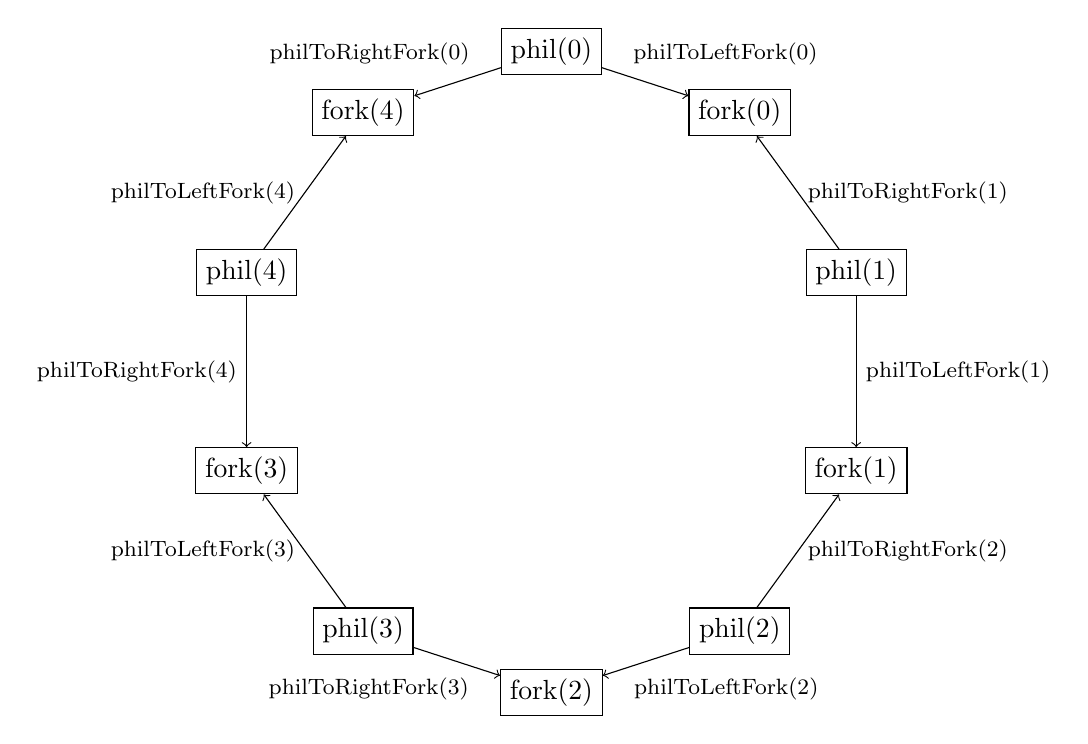
\begin{tikzpicture}
\foreach \i in {0,...,4} 
  \draw (90-72*\i: \r) node[draw] (phil\i) {\scalashape phil(\i)}; 
\foreach \i in {0,...,4} 
  \draw (54-72*\i: \r) node[draw] (fork\i) {\scalashape fork(\i)}; 
%
\draw[->] (phil0) -- node[above right, near start] 
  {\scalashape\footnotesize philToLeftFork(0)} (fork0);
\draw[->] (phil1) -- node[right] 
  {\scalashape\footnotesize philToLeftFork(1)} (fork1);
\draw[->] (phil2) -- node[below right, near end] 
  {\scalashape\footnotesize philToLeftFork(2)} (fork2);
\draw[->] (phil3) -- node[left] 
  {\scalashape\footnotesize philToLeftFork(3)\ } (fork3);
\draw[->] (phil4) -- node[left] 
  {\scalashape\footnotesize philToLeftFork(4)\ } (fork4);
%
\draw[->] (phil0) -- node[above left, near start]
  {\scalashape\footnotesize philToRightFork(0)} (fork4);
\draw[->] (phil1) -- node[right]
  {\scalashape\footnotesize philToRightFork(1)} (fork0);
\draw[->] (phil2) -- node[right]
  {\scalashape\footnotesize philToRightFork(2)} (fork1);
\draw[->] (phil3) -- node[below left, near end]
  {\scalashape\footnotesize philToRightFork(3)} (fork2);
\draw[->] (phil4) -- node[left]
  {\scalashape\footnotesize philToRightFork(4)} (fork3);
\end{tikzpicture}
\end{center}

%%%%%

\begin{scala}
  /** The complete system. */ 
  def system = {
    val philToLeftFork, philToRightFork = Array.fill(N)(new SyncChan[Cmd])
    // £philToLeftFork(i)£ is from £phil(i)£ to £fork(i)£;
    // £philToRightFork(i)£ is from £phil(i)£ to £fork($(\sm i-1) \bmod \sm N$)£.
    val allPhils = || ( 
      for (i <- 0 until N) yield phil(i, philToLeftFork(i), philToRightFork(i))
    )
    val allForks = || ( 
      for (i <- 0 until N) yield
        fork(i, philToRightFork((i+1)%N), philToLeftFork(i))
    )
    allPhils || allForks
  }

  /** Run the system. */
  def main(args : Array[String]) = run(system)
\end{scala}
\caption{The Dining Philosophers example (part 2).}
\label{fig:dining-philosophers-2}
\end{figure}

%%%%%%%%%%%

It is important that we use \emph{synchronous} channels: we need each
philosopher and fork to synchronise on relevant actions. 

When we run the system, sometimes it deadlocks almost immediately.  A typical
deadlocking trace is:
%
\begin{scala}
1 sits,  0 sits,  4 sits,  2 sits,  1 picks up left fork, 3 sits,  0 picks up left fork,  
4 picks up left fork, 2 picks up left fork,  3 picks up left fork
\end{scala}
%
Each philosopher sits down and picks up their left fork (in some order).  At
this point, each philosopher is trying to pick up its right fork, i.e.~to send
a |Pick| message on its |right| channel; however, the corresponding fork is
not willing to receive that message.  This means that the system is
deadlocked.

Recall that typing \texttt{Ctrl}+$\backslash$ (control and backslash) produces
a thread dump.  This gives the line number in the code where each thread is
stuck, so can help to understand the deadlock.

However, sometimes when we run the system, it runs for a very long time
without deadlocking.  In fact, I chose the delays in the simulations of the
basic actions so that the system deadlocks about half the time.  Different
choices for these delays would have caused the system to deadlock on nearly
every run, or hardly ever.  In some ways, the latter situation is worse: it is
likely that the potential deadlock would not be found by routine testing, but
that it would occur only when the system is deployed.

%%%%%%%%%%%%%%%%%%%%%%%%%%%%%%%%%%%%%%%%%%%%%%%%%%%%%%%%%%%%%%%%%

\section{Logging and Debugging}

In the above simulation, we used |println| statements so that we could
understand what happened.  However, this style is often not convenient when
tracking down bugs.  Normally, a better way to is to use logging.

The SCL class |Log| provides log objects.
%
A new log storing events of type~|A|, suitable for |p| threads,
can be defined by
\begin{scala}
  val log = new Log[A](p)
\end{scala}
%
This provides operations
%
\begin{itemize}
\item |def add(me: Int, x: A)|, which adds |x| to the log,
performed by thread~|me|;

\item |def get: Array[A]|, which gets the contents of the log;

\item |def toFile(fname: String = "/tmp/logFile")|, which writes the contents
  of the log to the file~|fname| (with a default of \texttt{/tmp/logFile}).
\end{itemize}

The code below shows how we can use logging in the dining philosophers
example.
%
\begin{scala}
  val log = new Log[String](N)
 
  def phil(me: Int, left: !![Cmd], right: !![Cmd]) = thread(s"Phil $me"){
    repeat{
      think()
      log.add(me, s"$me sits"); pause()
      left!Pick; log.add(me, s"$me picks up left fork"); pause()
      right!Pick; log.add(me, s"$me picks up right fork"); pause()
      log.add(me, s"$me eats"); eat()
      left!Drop; pause(); right!Drop; pause()
      log.add(me, s"$me leaves")
      if(me == 0) print(".")
    }
  }
\end{scala}
%
(I have arranged for philosopher~|0| to print a dot on each iteration, so we
can tell whether the system is making progress.)

In many scenarios, when the system terminates, we can either write the log to
a file, or analyse the log using some code.  However, this won't work when the
system deadlocks.  Instead, we need to insert a hook that will arrange for the
log to write itself to a file when the user interrupts the program.  This can
be done with the |writeToFileOnShutdown| method:
%
\begin{scala}
  def main(args: Array[String]) = {
    log.writeToFileOnShutdown("philsLog.txt"); run(system)
  }
\end{scala}

Logging is a general technique that can help with debugging.  However, there
is a wrinkle concerning its usage.
%
Internally, each thread uses its own thread-local log, to avoid race
conditions, and for efficiency.  Each logged value is stored in the relevant
thread-local logs, together with a timestamp (more precisely, the time elapsed
since the |Log| object was created, to avoid problems with timestamp
wrap-around).
%
The |get| operation merges the thread-local logs according to
timestamps.

Using timestamps in this way assumes that the clocks are loosely synchronised
across cores, and that the granularity of the clocks is sufficiently fine, so
that if one |add| event logically happens before another (i.e.~according to
the~$\prec$ relation), the former receives a strictly smaller timestamp.

The above assumption seems to be sound in Linux, but not in Windows.  If you
must use Windows, the class |SharedLog| provides the same interface.  However,
it will give worse performance.  Further, it might affect the likelihood of
detecting bugs: I have experienced bugs that would appear when no logging was
performed, or when the timestamp-based log was used; but logging with
something equivalent to |SharedLog| affected the speed of threads sufficiently
that the bug would no longer appear in a reasonable time!


